% ── ZFC axiom presentation (Set Theory background) ──────────────────────────
% Side-by-side layout: prose + formula on the left, an illustration on the
% right (mirrors a "numbered axiom with a small picture" style).
%   #1 = axiom body (name, description, \axiomeq formula, side conditions)
%   #2 = illustration: a tikzpicture, or \axiomfigtodo while it is unfinished.
% The number top-aligns with the first line of the body, while the illustration
% is vertically centered against the whole body block.
\newsavebox{\axiomtxtbox}
\newsavebox{\axiomfgbox}
\newcommand{\axiomlayout}[2]{%
  \sbox{\axiomtxtbox}{\begin{minipage}[t]{0.66\linewidth}#1\end{minipage}}%
  \sbox{\axiomfgbox}{#2}%
  \usebox{\axiomtxtbox}%
  \hfill
  \makebox[0.30\linewidth][r]{%
    \raisebox{\dimexpr 0.5\ht\axiomtxtbox - 0.5\dp\axiomtxtbox
                       - 0.5\ht\axiomfgbox + 0.5\dp\axiomfgbox\relax}%
             {\usebox{\axiomfgbox}}%
  }%
}
% Displayed axiom formula that auto-shrinks to the column width only if it would
% otherwise overflow the (narrow) left column; otherwise typeset at full size.
\newlength{\axiomeqwd}
\newcommand{\axiomeq}[1]{%
  \par\nobreak\vspace{3pt}%
  \settowidth{\axiomeqwd}{\ensuremath{\displaystyle #1}}%
  \makebox[\linewidth]{%
    \ifdim\axiomeqwd>\linewidth
      \resizebox{\linewidth}{!}{\ensuremath{\displaystyle #1}}%
    \else
      \ensuremath{\displaystyle #1}%
    \fi}%
  \par\vspace{3pt}%
}
% Placeholder illustration, shown until the real picture is drawn.
\newcommand{\axiomfigtodo}{%
  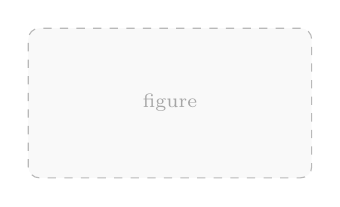
\begin{tikzpicture}
    \node[draw, dashed, rounded corners, gray!55, fill=gray!5,
          minimum width=3.6cm, minimum height=1.9cm, inner sep=0pt,
          font=\scriptsize, text=gray!70] {figure};
  \end{tikzpicture}%
}

% ── Illustrations for the ZFC axioms (manuscript palette) ───────────────────
\tikzset{
  axcard/.style={rounded corners=3pt, draw=venn-dark!45, fill=beige,
                 line width=0.5pt, minimum width=3.6cm, minimum height=1.9cm, inner sep=0pt},
  axset/.style={circle, draw=green!70!black, fill=green!20, line width=0.7pt},
  axsetb/.style={circle, draw=green!62!black, fill=green!13, line width=0.55pt},
  axsetc/.style={circle, draw=green!55!black, fill=green!7, line width=0.45pt},
  axsetbox/.style={draw=green!70!black, fill=green!20, line width=0.7pt},
  axarr/.style={-{Stealth[length=4pt,width=3.5pt]}, draw=dark-blue, line width=0.9pt,
                shorten <=3pt, shorten >=3pt},
  axarrp/.style={-{Stealth[length=4pt,width=3.5pt]}, draw=pink, line width=1.1pt,
                shorten <=3pt, shorten >=3pt},
}
\newcommand{\shC}[2][green]{\fill[#1] (#2) circle (1.7pt);}
\newcommand{\shS}[2][orange]{\fill[#1] ($(#2)+(-1.6pt,-1.6pt)$) rectangle ($(#2)+(1.6pt,1.6pt)$);}
\newcommand{\shT}[2][pink]{\fill[#1] ($(#2)+(0,2.1pt)$) -- ($(#2)+(-1.9pt,-1.5pt)$) -- ($(#2)+(1.9pt,-1.5pt)$) -- cycle;}
\newcommand{\sdot}[2][green]{\fill[#1] (#2) circle (1.5pt);}

\newcommand{\axfigExt}{\begin{tikzpicture}
  \node[axcard]{};
  \node[axset, minimum size=0.98cm] at (-0.95,0){};
  \node[axset, minimum size=0.98cm] at ( 0.95,0){};
  \node[dark-blue, font=\large] at (0,0){$=$};
  \shC[green]{-1.1,0.15}\shS[orange]{-0.8,0.13}\shT[pink]{-0.96,-0.18}
  \shS[orange]{0.82,0.15}\shT[pink]{1.1,0.02}\shC[green]{0.92,-0.17}
\end{tikzpicture}}

\newcommand{\axfigPair}{\begin{tikzpicture}
  \node[axcard]{};
  \node[axset, minimum size=0.62cm] (pa) at (-1.12,0.44){};
  \shC[orange]{-1.23,0.44}\shT[pink]{-1.01,0.44}
  \node[axset, minimum size=0.7cm] (pb) at (-1.06,-0.42){};
  \shC[green]{-1.2,-0.35}\shS[pink]{-0.94,-0.33}\shT[orange]{-1.07,-0.55}
  \node[fit=(pa)(pb), inner sep=0pt] (L) {};
  \node[axsetbox, rounded corners=0.5cm, minimum width=1.0cm, minimum height=1.62cm] (R) at (0.98,0){};
  \node[axsetb, minimum size=0.6cm] at (0.98,0.4){};
  \shC[orange]{0.87,0.4}\shT[pink]{1.09,0.4}
  \node[axsetb, minimum size=0.68cm] at (0.98,-0.4){};
  \shC[green]{0.84,-0.33}\shS[pink]{1.1,-0.31}\shT[orange]{0.96,-0.54}
  \draw[axarr] (L.east |- R) -- (R.west);
\end{tikzpicture}}

\newcommand{\axfigUnion}{\begin{tikzpicture}
  \node[axcard]{};
  \node[axsetbox, rounded corners=0.46cm, minimum width=0.92cm, minimum height=1.42cm] (L) at (-1.02,0){};
  \node[axsetb, minimum size=0.58cm] at (-1.02,0.36){};
  \shC[green]{-1.13,0.36}\shT[orange]{-0.91,0.36}
  \node[axsetb, minimum size=0.46cm] at (-1.02,-0.38){};
  \shS[pink]{-1.02,-0.38}
  \node[axset, minimum size=1.08cm] (R) at (1.02,0){};
  \shC[green]{0.86,0.17}\shT[orange]{1.2,0.12}\shS[pink]{1.04,-0.2}
  \draw[axarr] (L.east |- R) -- (R.west);
\end{tikzpicture}}

\newcommand{\axfigPow}{\begin{tikzpicture}
  \node[axcard]{};
  \node[axset, minimum size=0.72cm] (L) at (-0.95,0){};
  \shC[green]{-1.06,0}\shS[orange]{-0.84,0}
  \node[axset, minimum size=1.4cm] (R) at (1.0,0){};
  \node[axsetb, minimum size=0.42cm] at (0.72,0.3){};
  \node[axsetb, minimum size=0.42cm] at (1.28,0.3){}; \shC[green]{1.28,0.3}
  \node[axsetb, minimum size=0.42cm] at (0.72,-0.3){}; \shS[orange]{0.72,-0.3}
  \node[axsetb, minimum size=0.42cm] at (1.28,-0.3){}; \shC[green]{1.21,-0.3}\shS[orange]{1.35,-0.3}
  \draw[axarr] (L.east |- R) -- (R.west);
\end{tikzpicture}}

\newcommand{\axfigInf}{\begin{tikzpicture}
  \node[axcard]{};
  \node[axsetbox, rounded corners=0.56cm, minimum width=2.9cm, minimum height=1.12cm] at (0,0){};
  \node[green!60!black, font=\large] at (0,0.74){$\infty$};
  % 0 = empty set
  \node[axsetb, minimum size=0.2cm] at (-1.18,0){};
  % 1 = { empty set }
  \node[axsetb, minimum size=0.5cm] at (-0.66,0){};
  \node[axsetc, minimum size=0.2cm] at (-0.66,0){};
  % 2 = { empty set, { empty set } }
  \node[axsetb, minimum size=0.98cm] at (0.2,0){};
  \node[axsetc, minimum size=0.2cm] at (-0.04,0){};
  \node[axsetc, minimum size=0.45cm] at (0.4,0){};
  \node[axsetc, minimum size=0.1cm] at (0.4,0){};
  % continuation (dots drawn manually so they sit on the vertical centre)
  \fill[dark-blue] (1.0,0) circle (0.7pt);
  \fill[dark-blue] (1.12,0) circle (0.7pt);
  \fill[dark-blue] (1.24,0) circle (0.7pt);
\end{tikzpicture}}

\newcommand{\axfigReg}{\begin{tikzpicture}
  \node[axcard]{};
  \node[axset, minimum size=0.72cm] at (0,0){};
  \node[axsetb, minimum size=0.36cm] at (0,0){};
  \draw[-{Stealth[length=4pt,width=3.5pt]}, draw=dark-blue, line width=0.9pt] (0.33,0.24) to[out=20,in=-20,looseness=5.5] (0.33,-0.24);
  \draw[pink, line width=1.5pt] (0,0) circle (0.66);
  \draw[pink, line width=1.5pt] (-0.47,0.47) -- (0.47,-0.47);
\end{tikzpicture}}

\newcommand{\axfigSep}{\begin{tikzpicture}
  \node[axcard]{};
  \node[axset, minimum size=1.16cm] (L) at (-1.0,0){};
  \shC[pink]{-1.21,0.24}\shT[pink]{-0.81,0.26}\shS[pink]{-1.0,-0.26}
  \shC[green]{-0.79,-0.06}\shT[orange]{-1.19,-0.12}\shS[blue]{-0.99,0.04}
  \node[axset, minimum size=0.84cm] (R) at (1.0,0){};
  \shC[pink]{0.88,0.17}\shT[pink]{1.15,0.13}\shS[pink]{0.98,-0.18}
  \draw[axarrp] (L.east |- R) -- (R.west);
\end{tikzpicture}}

\newcommand{\axfigRepl}{\begin{tikzpicture}
  \node[axcard]{};
  \node[axset, minimum size=1.0cm] (L) at (-1.15,0){};
  \shC[green]{-1.15,0.26}\shC[orange]{-1.15,0}\shC[pink]{-1.15,-0.26}
  \node[axset, minimum size=1.0cm] (R) at (1.15,0){};
  \shS[green]{1.15,0.26}\shS[orange]{1.15,0}\shS[pink]{1.15,-0.26}
  \draw[axarr] (L.east |- R) -- (R.west) coordinate[midway] (m);
  \draw[dark-blue, line width=0.4pt] ($(m)+(-0.24,0.34)$) circle (2.3pt);
  \node[dark-blue, font=\scriptsize] at ($(m)+(0,0.34)$) {$\mapsto$};
  \draw[dark-blue, line width=0.4pt] ($(m)+(0.24,0.34)+(-2.3pt,-2.3pt)$) rectangle ($(m)+(0.24,0.34)+(2.3pt,2.3pt)$);
\end{tikzpicture}}

\newcommand{\axfigChoice}{\begin{tikzpicture}
  \node[axcard]{};
  \node[axset, minimum size=0.52cm] (c1) at (-1.02,0.44){};
  \shC[pink]{-1.13,0.44}\shC[green]{-0.91,0.44}
  \node[axset, minimum size=0.52cm] (c2) at (-1.45,-0.3){};
  \shT[orange]{-1.55,-0.3}\shT[pink]{-1.35,-0.3}
  \node[axset, minimum size=0.52cm] (c3) at (-0.59,-0.3){};
  \shS[green]{-0.69,-0.3}\shS[pink]{-0.49,-0.3}
  \node[fit=(c1)(c2)(c3), inner sep=0pt] (L) {};
  \node[axset, minimum size=0.92cm] (R) at (1.0,0){};
  \shC[pink]{1.0,0.18}\shT[pink]{0.84,-0.16}\shS[pink]{1.16,-0.16}
  \draw[axarr] (L.east |- R) -- (R.west);
\end{tikzpicture}}
